\documentclass[../Main.tex]{subfiles}

\begin{document}
\section{Homomorphisms}
Informally, a homomorphism is a type of map that respects the structure of a group. The way in which it does this is now defined:
\begin{definition}{Homomorphism}
    A homomorphism $\phi : G \mapsto H$, where $G$ and $H$ are groups, is a function that has the extra property $\phi(g_1 \cdot g_2) = \phi(g_1) \cdot \phi(g_2)$, where $g_1, g_2 \in G$.
\end{definition}
\begin{examples}[Examples of homomorphisms]{}
    \item The trivial homomorphism $\phi : G \mapsto H, \phi(g) = e$
    \item The inclusion homomorphism: for a subgroup $H \leq G$, $i : H \mapsto G, i(h) = h \in G$.
\end{examples}
We would also like some useful properties of homomorphisms:
\begin{propositions}{
        \label{propHismFundamentals}
        If $\phi : G \mapsto H$ is a homomorphism,
    }
    \item $\phi(e_G) = e_H$ \label{propIdentitiesMap}
    \item $\phi(g^{-1}) = (\phi(g))^{-1}$ \label{propInversesmap}
\end{propositions}
\begin{proof}
    \begin{enumerate}
        \item Identity maps to identity:
        \begin{align*}
            e_H &= \phi(e_G)^{-1} \cdot \phi(e_G) \\
            &= \phi(e_G)^{-1} \cdot \phi(e_g \cdot e_G) \\
            &= \phi(e_G)^{-1} \cdot \phi(e_G) \cdot \phi(e_G) \\
            &= e_H \cdot \phi(e_G) \\
            &= \phi(e_G)
        \end{align*}
        \item Inverses map to inverses:
        \begin{align*}
            \phi(g^{-1}) \cdot \phi(g) &= \phi(g^{-1} \cdot g) \\
            &= \phi(e_G) \\
            &= e_H \text{ by proposition~\ref{propIdentitiesMap}}
        \end{align*}
        So $\phi(g)^{-1} = \phi(g^{-1})$ by uniqueness of inverses.
    \end{enumerate}
\end{proof}
\begin{example}
    \label{exZnCnHism}
    Consider the groups:
    \begin{eqnarray*}
        C_n = \subsetselect{z \in C}{z^n = 1} \text{ under multiplication} \\
        \Z_n = \subsetselect{k \in \Z}{0 \leq k < n} \text{ under modulo addition}
    \end{eqnarray*}
    Then we define the map:
    \begin{align*}
        \phi : \Z_n &\mapsto C_n \\
        k &\mapsto e^{2\pi\frac{k}{n}}
    \end{align*}
    In $\Z_n$, the group operation of modulo addition, $+_n$, has $k +_n l = (k + l) - np, n \in \N$.
    \begin{align*}
        \phi(k +_n l) &= e^{2\pi\frac{k +_n l}{n}} \\
        &= e^{2\pi\frac{k + l - np}{n}} \\
        &= e^{2\pi\frac{k + l}{n} + 2\pi p} \\
        &= e^{2\pi\frac{k+l}{n}} \times e^{2\pi p} \\
        &= e^{2\pi\frac{k+l}{n}} \times 1 \\
        &= e^{2\pi\frac{k}{n}} \times e^{2\pi\frac{l}{n}} \\
        &= \phi(k) \times \phi(l)
    \end{align*}
    And therefore $\phi$ is a homomorphism.
\end{example}
\subsection{Isomorphisms}
We now have a convenient way to say that groups are equivalent:
\begin{definition}{Isomorphism}
    An \underline{isomorphism} $G \mapsto H$ is a homomorphism that is bijective. If an isomorphism exists then we say $G$ and $H$ are isomorphic, $G \cong H$.
\end{definition}
We can also use some important results without proof:
\begin{propositions}{
        If $\phi : G \mapsto H$ is a homomorphism,
    }
    \item $\phi^{-1}$ exists then is a homomorphism
    \item If further $\psi : H \mapsto K$ is a homomorphism then the composition $\psi \cdot \phi$ is a homomorphism
    \item Isomorphism, $\cong$, is an equivalence relation, so $G \cong H \Leftrightarrow H \cong G$, and $G \cong H \cong K \implies G \cong K$.
\end{propositions}
\subsection{Image and Kernel}
The image and kernel are defined similarly to in IA Numbers and Sets:
\begin{definition}{Image}
    The \underline{image} of a homomorphism $\phi : G \mapsto H$ is $\im{\phi} = \subsetselect{h \in H}{\exists g \in G \text{ such that } \phi(G) = h}$. It is all the elements in $H$ that are mapped to by elements of $G$.
\end{definition}
\begin{definition}{Kernel}
    The \underline{kernel} of a homomorphism $\phi : G \mapsto H$ is $\ker{\phi} = \subsetselect{g \in G}{\phi(g) = e_H}$. It is all the elements of $G$ that map to the identity in $H$.
\end{definition}
\begin{propositions}{
        For a homomorphism $\phi : G \mapsto H$,
    }
    \item $\im{\phi} \leq H$
    \item $\ker{\phi} \leq G$
\end{propositions}
\begin{proof}
    \begin{enumerate}
        \item Image is a subgroup of codomain group:
        We must have that the identity is is the image, since $\phi(e_G) = e_H$ by Proposition~\ref{propIdentitiesMap}, and that the inverse of any element in the image is also in the image by Proposition~\ref{propInversesmap}. Therefore, we simply the image to be closed under the group operation, which follows directly from the definition of a homomorphism.
        \item Kernel is a subgroup of domain group:
        Since $\phi(e_G) = e_H, e_G \in \ker{\phi}$.\par
        Also, if $g_1, g_2 \in \ker{\phi}$,
        \begin{align*}
            \phi(g_1 \cdot g_2) &= \phi(g_1) \cdot \phi(g_2) \\
            &= e_H \cdot e_H \\
            &= e_H
        \end{align*}
        So for any two elements $g_1, g_2 \in \ker{\phi}$, $g_1 \cdot g_2 \in \ker{\phi}$.\par
        If $g \in \ker{\phi}$, $\phi(g^{-1}) = \phi(g)^{-1} = e_H^{-1} = e_H$, so if $g \in \ker{\phi}, g^{-1} \in \ker{\phi}$.\par
        $\therefore \ker{\phi} \leq G$.
    \end{enumerate}
\end{proof}
We inherit the standard definitions of surjectivity and injectivity from Part IA Numbers and Sets. However, we can use the properties of groups and homomorphisms to greatly simplify the tests for these properties:
\begin{proposition}
    A homomorphism $\phi : G \mapsto H$ is injective if and only if $\ker{\phi} = \{e_G\}$.
    \label{propInjectivityTrivialKer}
\end{proposition}
\begin{proof}
    \begin{proofdirection}{$\Rightarrow$}{Assume $\phi$ is injective.}
        But this means that at most one element in $G$ can map to the identity in $H$. Therefore, the kernel must contain one element, and by Proposition~\ref{propIdentitiesMap}, this must be $e_G$.
    \end{proofdirection}
    \begin{proofdirection}{$\Leftarrow$}{Assume $\ker{\phi} = \{e_G\}$}
        Suppose $\phi(g_1) = \phi(g_2)$.
        \begin{align*}
            \phi(g_1 g_2^{-1}) &= \phi(g_1) \cdot \phi(g_2^{-1}) \\ 
            &= \phi(g_1) \cdot \phi(g_2)^{-1} \\
            &= e_H
        \end{align*}
        So then $g_1 g_2^{-1} \in \ker{\phi}$, which means $g_1 g_2^{-1} = e_G$ by assumption.\par
        But by uniqueness of inverses, $g_2^{-1} = g_1^{-1}$, so $g_1 = g_2$. That is, $\phi$ is injective.
    \end{proofdirection}
\end{proof}
We also have a condition for surjectivity from IA Numbers and Sets: $\phi : G \mapsto H$ is surjective if and only if $\im{\phi} = H$. So combining these gives us the conditions for bijectivity.
\section{The Cyclic Group}
\begin{definition}{Cyclic group}
    A group $G$ is \underline{cyclic} if there exists an element $g$ such that:
    \begin{equation*}
        G = \subsetselect{g^k}{k \in \Z}
    \end{equation*}    
    That is, $g$ generates $G$. $\langle g \rangle = G$.
\end{definition}
\begin{examples}{}
    \item $C_n = \subsetselect{z \in \C}{z^n = 1}$ is a cyclic group, with generator $e^{\frac{2i\pi}{n}}$
    \item $\Z$ under addition is an infinite cyclic group with generator $1$.
    \item $Z_n$ is cyclic, $Z_n \cong C_n$.
\end{examples}
We can also classify all the cyclic groups.
\begin{theorem}
    If $G$ is a cyclic group then either $G \cong C_n$ or $G \cong \Z$.
\end{theorem}
\begin{proof}
    Let $G$ be a cyclic group with generator $g$. Define the set:
    \begin{equation*}
        S = \subsetselect{k \in \N}{g^k = e}
    \end{equation*}
    \begin{case}{$S = \emptyset$}
        We want to show that $G \cong \Z$. Define a map:
        \begin{align*}
            \phi : \Z &\mapsto G \\
            k &\mapsto g^k
        \end{align*}
        Note that:
        \begin{align*}
            \phi(k+l) &= g^{k + l} \\
            &= g^k g^l \\
            &= \phi(k) \phi(l)
        \end{align*}
        so $\phi$ is a homomorphism. We also have surjectivity due to the definition of $g$ as a generator. For injectivity, by proposition~\ref{propInjectivityTrivialKer}, we only need to prove that $\ker{\phi}$ is trivial.\par
        Suppose, on the contrary, that there is an integer $h \neq 0$ in the kernel. But then $h \in S$. \contradiction $S = \emptyset$ by assumption.\par
        So now $\phi$ is an isomorphism, so $G \cong \Z$.
    \end{case}
    \begin{case}{$S \neq \emptyset$}
        $S$ is non-empty, so by the well-ordering principle we take the least element of $S$ and label it $n$. Now define the map:
        \begin{align*}
            \phi : \Z_n &\mapsto G \\
            k &\mapsto g^k
        \end{align*}
        We have seen that this map is a homomorphism in example~\ref{exZnCnHism}. We can argue again that $\phi$ is surjective because $G$ is generated by $g$. Injectivity again requires proving a trivial $\ker{\phi}$:\par
        Suppose there exists some $h \neq 0$ in the kernel. Then we have $0 < h < n$, and $g^h = e$. This implies $h \in S$ but $h < n$ \contradiction~$n$ was chosen to be the smallest by well-ordering principle.\par
        So $\ker{\phi}$ is trivial and $\phi$ is injective. We have a bijective homomorphism so $G \cong \Z_n \cong C_n$.
    \end{case}
\end{proof}
\begin{remark}
    We may also write $C_\infty \cong \Z$.
\end{remark}
We now have a fairly simple test for isomorphism to a cyclic group: if $G$ is generated by one element $g$, then we have $G \cong \Z$ if it is an infinite group, or $G \cong C_n$ if it is a finite group with order $n$.
\section{The Dihedral Group}
We also consider another example of a group, with a nice geometrical interpretation.\par
Let $X_n \subset \C$ be the set of vertices of the regular $n$-gon. That is,
\begin{equation}
    X_n = \subsetselect{e^{2i\pi\frac{k}{n}}}{0\leq k < n}
    \label{eqnXn}
\end{equation}
Then we define:
\begin{definition}{Dihedral group}
    The $n$th dihedral group, $D_{2n}$, is defined to be the group of isometries of $X_n, \Isom{(X_n)}$.
\end{definition}
We would like to understand the elements of $D_{2n}$, and first some lemmas are needed.
\begin{lemma}[Kite lemma]
    Let $x_1, x_2, y_1, y_2 \in \C$. Suppose that $|y_1 - x_1| = |y_2 - x_2|$ and $|y_1 - x_2| = |y_2 - x_1|$.\par
    Then the lines $x_2 - x_1$ and $y_2 - y_1$ are perpendicular.
\end{lemma}
Geometrically, this is:
\begin{center}
    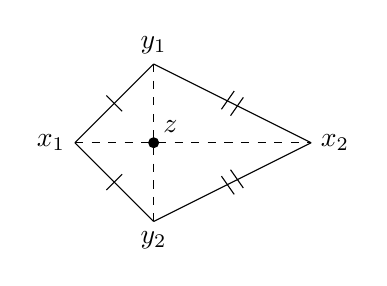
\begin{tikzpicture}
            \tikzset{
                singledash/.pic={
                    \draw (-1mm, 1mm) -- (1mm, -1mm);
                },
                doubledash/.pic={
                    \draw (-1.5mm, 0.5mm) -- (0.5mm, -1.5mm);
                    \draw (-0.5mm, 1.5mm) -- (1.5mm, -0.5mm);
                }
            }
        \draw (0, 0) node[anchor=east] (x1) {$x_1$} -- (1, 1) node[anchor=south] (y1) {$y_1$}
            pic[pos=0.5] {singledash};

        \draw (y1.south) -- (3, 0) node[anchor=west] (x2) {$x_2$}
            pic[pos=0.5, rotate=100] {doubledash};
        
        \draw (x2.west) -- (1, -1) node[anchor=north] (y2) {$y_2$}
            pic[pos=0.5, rotate=-10] {doubledash};
        
        \draw (y2.north) -- (x1.east)
            pic[pos=0.5, rotate=90] {singledash};
        \node[anchor=south west] (z) at (1, 0) {$z$};
        \fill (1, 0) circle (0.7mm);
        \draw[dashed] (x1) -- (x2);
        \draw[dashed] (y1) -- (y2);
    \end{tikzpicture}
\end{center}
If the marked lines have the same length, then the dashed lines are perpendicular.\par
\begin{proof}
    Consider the point $z$ at the intersection as in the diagram. By symmetry, the angles $x_1 z y_2$ and $x_2 z y_2$ are equal. But $y_1 y_2$ is a straight line so the two angles sum to $\pi$.\par
    And therefore each angle is $\frac{\pi}{2}$
\end{proof}
\begin{lemma}
    Let $f$ be an isometry of the complex plane. Then if there exist non-collinear points $x_1, x_2, x_3$ that have the property $f(x_i) = x_i$, then $f = Id_\C$.
\end{lemma}
\begin{proof}
    
\end{proof}
\end{document}